\section{SiPM module}
\subsection{SiPM detector}
The Silicon Photomultiplier (SiPM) is a single-photon sensitive sensor that has
performance characteristics comparable to a conventional ICCD/PMT/APD (Table ~\ref{tbl:sipm_comparison}).
with the practical advantages of a solid-state sensor. 


\begin{figure}[H]
\begin{center}
\begin{tabular}{ |c|c|c|c|c| } 
\hline
& ICCD & PMT & APD & SiPM  \\
\hline
Sensitivity & $\sim 10$ ph.e & 1 ph.e & $\sim 10$ ph.e & 1 ph.e  \\ 
\hline
Gain & $10^3-10^6$ & $10^6$ & 100-200 & $10^6$ \\ 
\hline
Dynamic Range & large & $\sim 10^3$  & lasrge & $\sim 10^3/mm^2$\\ 
\hline
Operating Voltage & $\sim 100 V$ & 1-2 kV & 100-500 V & 20-50 V\\ 
\hline
Efficiency at blue & 50\% & 20\% & 50\% & 30\% \\ 
\hline
Timing & $\sim 1 ms$ & $\sim 100 ps$ & $\sim ns$ & $\sim 30 ps$\\ 
\hline
\end{tabular}
\vspace{-5mm}
\caption{Specification of the LIDAR scanning system}
\label{tbl:sipm_comparison}
\end{center}
\end{figure}


It is formed of a summed array of closely-packed Single Photon Avalanche Photodiode (SPAD) sensors (Fig. \ref{fig:sipm_structure})

\begin{figure}[H]
\center{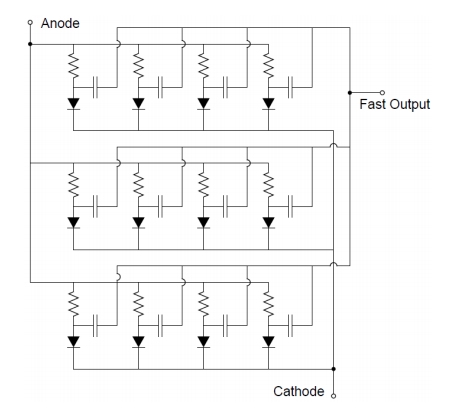
\includegraphics[width=0.5\linewidth]{sipm_structure}}
\caption{An SiPM consists of an array of microcells
(SPAD plus quench resistor) with summed output.}
\label{fig:sipm_structure}
\end{figure}


The SiPM is operated in Geiger-mode which enables high gain
(1x106), high detection efficiency (>50\%) and fast timing
(sub-ns rise times) at moderate bias (~30V). This is achieved by creating a high
field region in the diode that generates a self-perpetuating charge
avalanche when a photon is absorbed. Passive
quenching, is achieved through the use of a
series resistor which limits the current drawn by the diode during
breakdown. This lowers the reverse voltage seen by the diode to a
value below its breakdown voltage, thus halting the avalanche. The
diode then recharges back to the bias voltage, and is available to
detect subsequent photons.


Since the capacitance of the microcell will depend upon its area, the reset time will vary for different microcell sizes, with a 50mm
microcell SiPM having a significantly longer reset time and gain than a 10mm microcell SiPM.
Another one of the most important parameter is PDE (Photon Detection Efficiency). This is the product of the $QE\cdot AIP \cdot FF$, where $QE$ is quantum efficiency, $AIP$ is the avalanche initiation probability and $FF$ is the fill factor of the microcells.
The characteristics and PDE graph of the selected SiPM detector by Sensl are shown in the table \ref{tbl:sipm_characteristics} and figure \ref{fig:sipm_pde} correspondingly.


\begin{figure}[H]
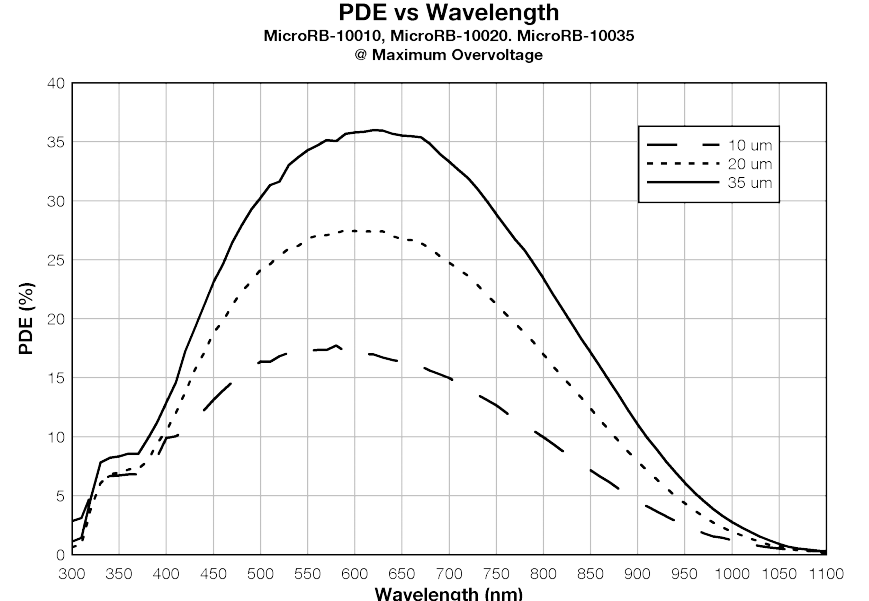
\includegraphics[width=1\linewidth]{sipm_pde}
\caption{PDE for different cell sizes.}
\label{fig:sipm_pde}
\end{figure}

\begin{table}[H]
\label{tbl:rfp_laser}
\begin{center}

\begin{tabular}{|p{0.2\linewidth}|p{0.3\linewidth}|}
\hline
Microsell size: & \textbf{$\pmb{35\; um}$}  \\ \hline
Gain: & \textbf{$\pmb{1.7 \cdot 10^6}$}  \\ \hline
PDE @ 905 nm: & \textbf{$\leq$ 10\%} \\\hline
Dark current rate: & \textbf{3.8 MHz} \\\hline
Dark current: & \textbf{1.5 uA} \\\hline
Rise time: & \textbf{3.7 ns} \\\hline
Recharge time: & \textbf{73 ns} \\  \hline
\end{tabular}
\vspace{-5mm}
\caption{Characteristics of the SiPM}
\label{tbl:sipm_characteristics}
\end{center}
\end{table}



In accordance with the characteristics of the detector, we can say that it is ideally suited for the LiDAR based on TOF technology. High gain and small rise time allows sigle-detection mode with high SNR, while small recharge time allow very high repetition rate, up to 10MHz.

Figure \ref{fig:sipm_pde} shows the SiPM experimental setup (left) and screenshot of the SiPM output after laser shooting (right), caught by the 2Gsa/s oscilloscope.


\begin{figure}[H]
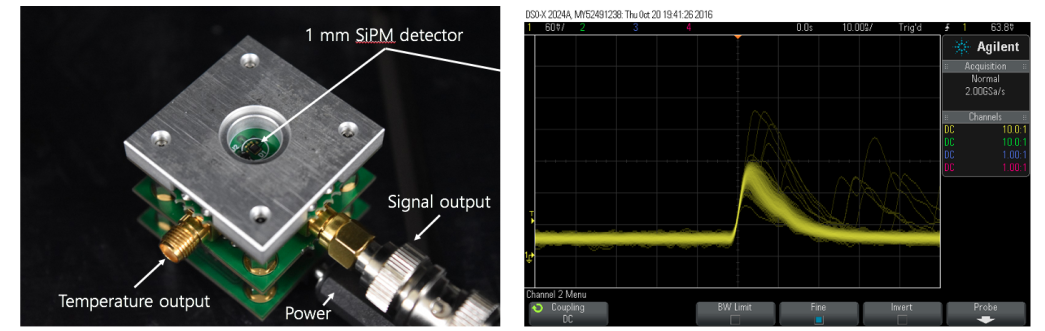
\includegraphics[width=1.05\linewidth]{sipm}
\caption{SiPM experimental setup (left) and output of SiPM after laser shooting (rigth).}
\label{fig:sipm_pde}
\end{figure}



\subsection{SiPM collimator}
Receiver optics is one of the most important in the whole system. It provides a specified FOV, minimizing noise. Our receiver aperture is limited by diameter of the MEMS, so it should not exceed 3.6mm.
Since we don't need wide FOV we are not suffering so much due to abberrations, thus the optical system consists of one aspherical lens to focus received signal to SiPM and a pinhole for cutting FOV according to eq:\ref{eq:sipm_FOV}.
FOV of SiPM should be big enough to cover laser beam, but at the same time should be quite small to decrease noise impact.


\begin{equation}\label{eq:sipm_FOV}
FOV = 2\cdot tan^{-1}(\frac{d}{2\cdot f})
\end{equation}
Where d is pinhole size, f is focal length.



\begin{figure}[h]
\begin{floatrow}
\ffigbox{
\center{
\includegraphics[width=0.65\linewidth]{ld_lens}} 
}{
  \caption{Aspheric lens used for SiPM collimator.}%
\label{fig:ld_lens} % or change caption location
}
\capbtabbox{

  \begin{tabular}{|M{4cm}|M{4cm}|}
\hline
Pinhole size: & \textbf{200 um} \\  \hline
Effective Focal length: & \textbf{4.5 mm} \\  \hline
Clear Aperture: & \textbf{3.7 mm} \\  \hline
Numerial aperture (NA): & \textbf{0.3} \\  \hline
Material: & \textbf{D-ZK3}  \\ \hline
Center Thickness: & \textbf{3.484 mm}  \\ \hline
Coating: & \textbf{ BBAR (600 - 1050 nm)} \\  \hline
\end{tabular}
}{%
\caption{Characteristics of optics for SiPM, bandpass filter should be improoved.}
\label{tbl:sipm_datasheet}
}
\end{floatrow}
\end{figure}


\begin{figure}[H]
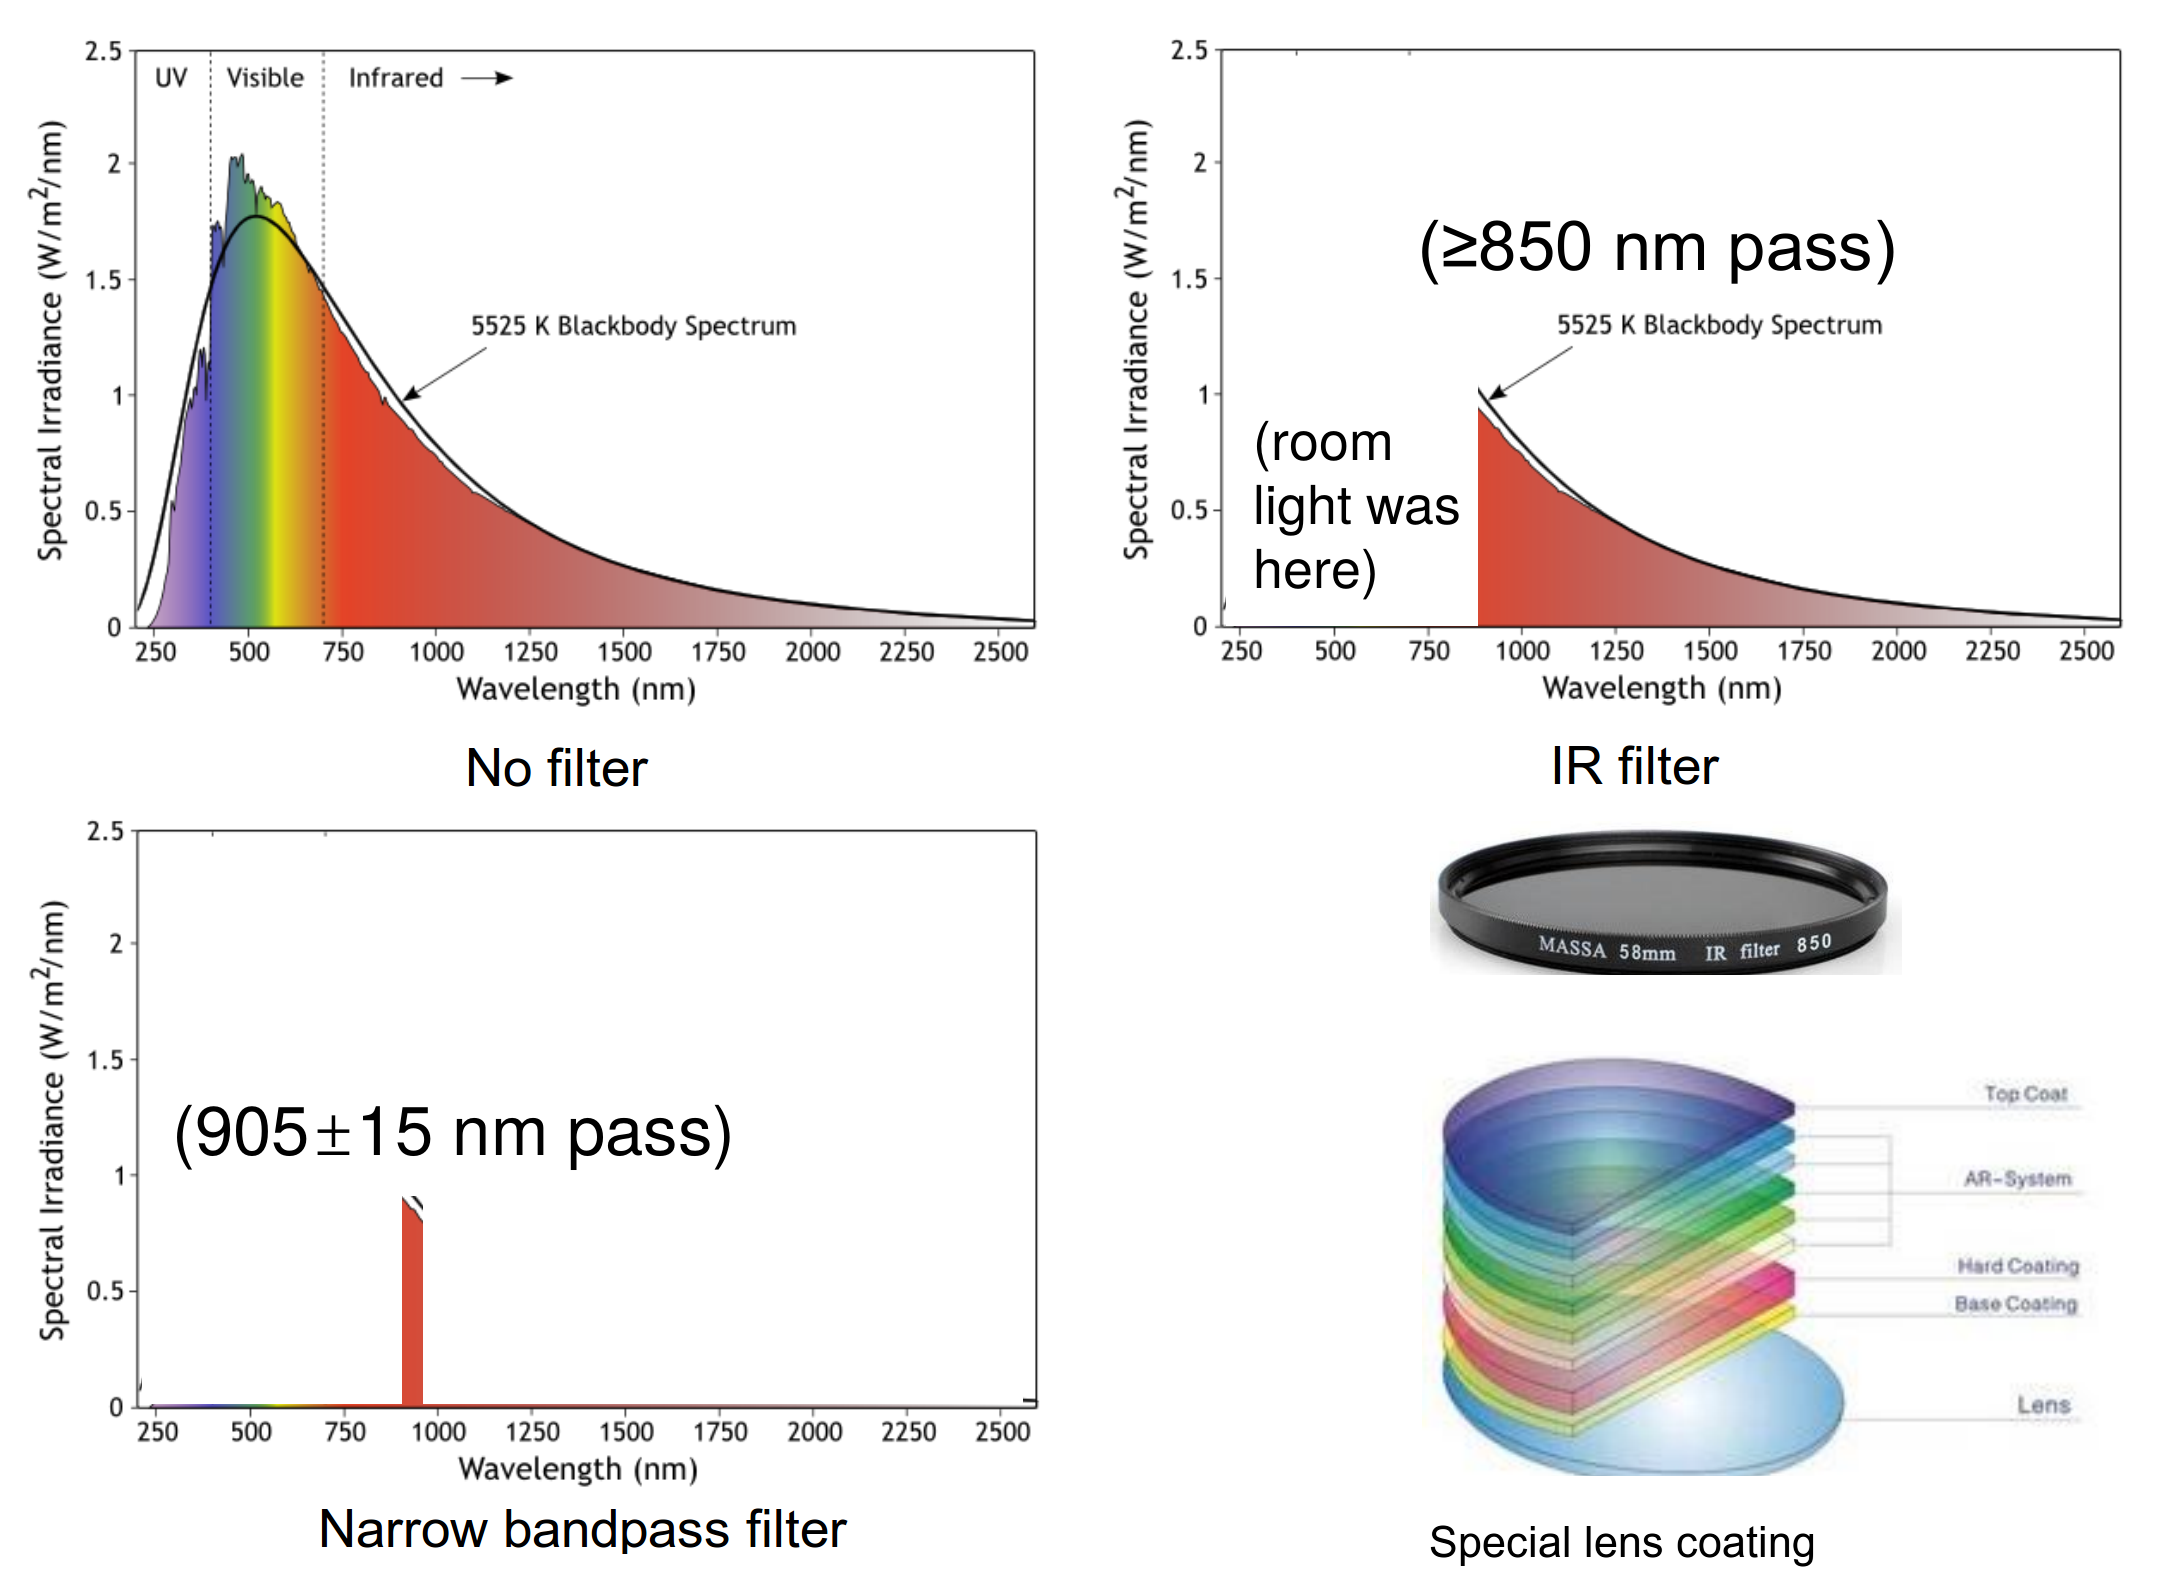
\includegraphics[width=1\linewidth]{coating}
\caption{Effect of the filter on the sun spectrum.}
\label{fig:coating}
\end{figure}

To make lidar could work in the daytime we should remove background as mush as we can, so an IR optical filter was built into the detector collimator. For sunny day the bandpass filter with 10nm bandwidth should be implemented, i.e by lens coating (Fig. \ref{fig:coating})



\begin{figure}[H]
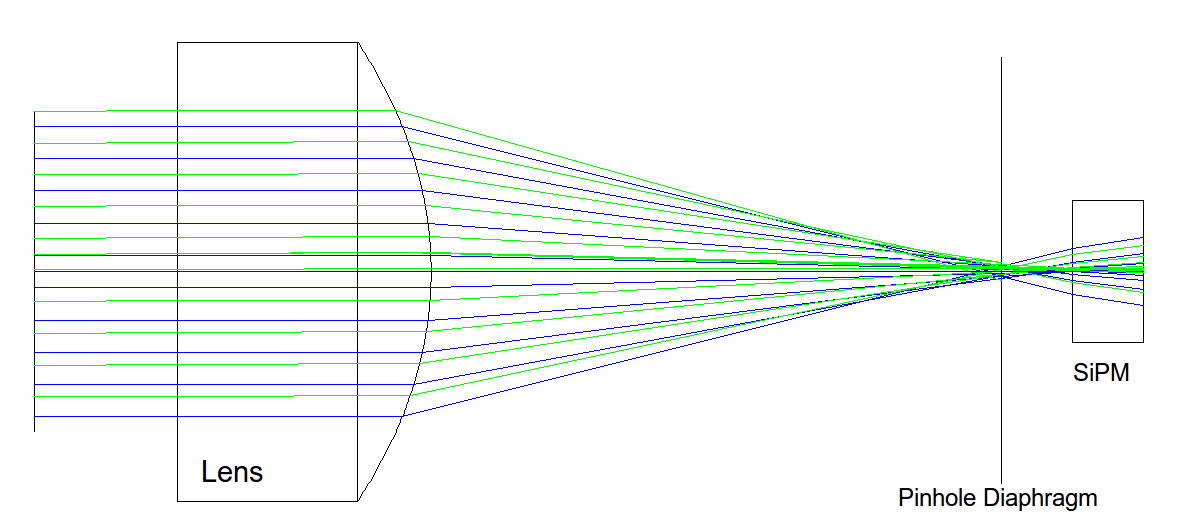
\includegraphics[width=0.7\linewidth]{sipm_zemax}
\caption{Zemax simulation of SiPM collimator.}
\label{fig:sipm_pde}
\end{figure}

Acoording to Zemax simulation, the FOV will be $2.8{^\circ}x2.8{^\circ}$,
thus we have tolerance for match both laser FoV and SiPM to cover fast axis of laser beam $(0.1{^\circ}x2.5{^\circ}$).



\subsection{Completed SiPM module}

The finished SiPM PCB is shown in the figure \ref{fig:sipm_PCB}
It consist of readout electronics for SiPM, laser driver and TDC chip, thereby integrates all functions of LiDAR itself: driving laser diode, generating high voltage for SiPM, readout and amplification of SiPM signal and measuring time delay between outgoing and return impulse.

\begin{figure}[h]
\center{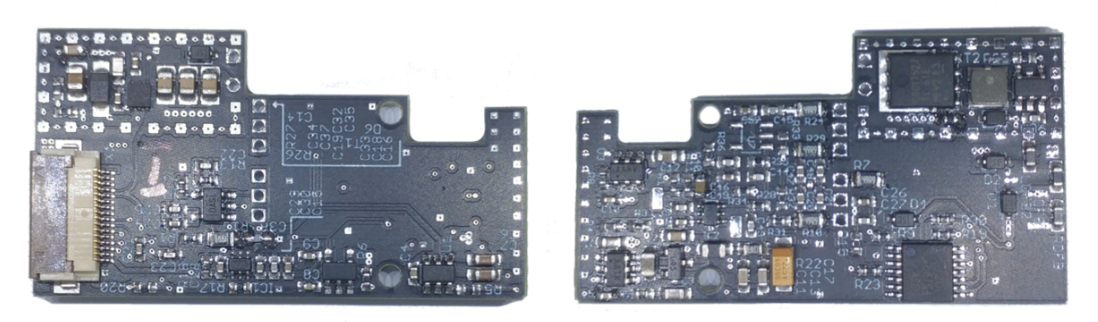
\includegraphics[width=0.85\linewidth]{sipm_PCB}} 
  \caption{Upper and lower side of SiPM PCB.}%
\label{fig:sipm_PCB} % or change caption location
\end{figure}

The assembled SiPM collimator with already attached SiPM to the bottom of tube is shown in figure \ref{fig:sipm_collimator}.
\begin{figure}[h]
\center{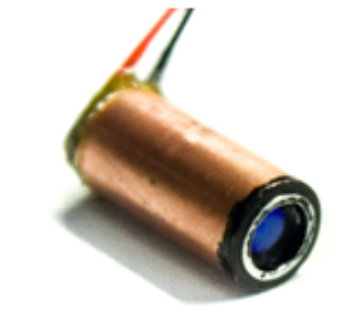
\includegraphics[width=0.3\linewidth]{sipm_collimator}} 
  \caption{Assembled SiPM collimator with integrated SiPM.}%
\label{fig:sipm_collimator} % or change caption location
\end{figure}




